\subsection{FreeRTOS Features Project}

This last project is designed to demonstrate how some of the features of FreeRTOS can be used. A timer, a semaphore and a queue are used to show how tasks can be synchronized and communicate with each other.

\subsubsection{Project Design}

\begin{figure}[ht]
    \centering
    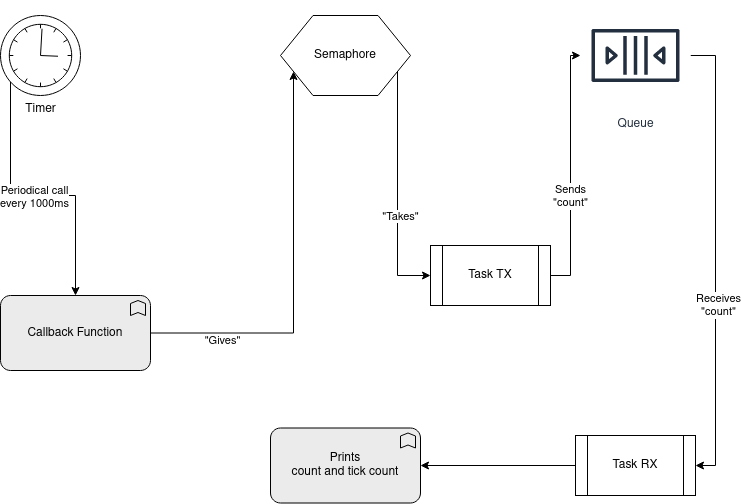
\includegraphics[width=0.8\textwidth]{images/projects/project_feature_schema.png}
    \caption{FreeRTOS Features Project Schema}
    \label{fig:project_feature_schema}
\end{figure}

The project is design as shown in the figure \ref{fig:project_feature_schema}. It works as follows:

\begin{description}
    \item[Timer] The timer is a software timer that is configured to expire periodically every 1000 milliseconds. Upon expiration, it triggers a callback function. The primary role of this callback function is to give a semaphore.
    \item[Semaphore] The semaphore is used to synchronize the operation of Task TX and the timer's callback function. When the timer's callback function is executed, it gives the semaphore. Task TX waits for the semaphore and performs its operation when it is given.
    \item[Task TX] Task TX is designed to demonstrate how a task can wait for a semaphore and perform an operation once the semaphore is given, it sends a value to a queue. This value is a counter that is incremented in each loop, serving as a simple demonstration of a task performing work in response to a semaphore.
    \item[Queue] The queue is used to send the value produced by Task TX to Task RX.
    \item[Task RX] Task RX is designed to demonstrate how tasks can wait for data on a queue and process it. It prints the received value and the current tick count. This demonstrates a task that consumes data produced by another task and the use of the system tick count to measure time in a real-time system.
\end{description}